% Póster en español. Compilar: uv run python make_figures.py y luego lualatex poster_es.tex dos veces.
% Shared preamble of poster_en.tex and poster_es.tex (A0 portrait).
\documentclass{article}
\usepackage[paperwidth=841mm,paperheight=1189mm,margin=0mm]{geometry}
\usepackage{fontspec}
\usepackage{unicode-math}
\usepackage[table]{xcolor}
\usepackage{graphicx}
\usepackage{tabularx}
\usepackage{array}
\usepackage{enumitem}
\usepackage{tcolorbox}
\tcbuselibrary{skins}
\usepackage{tikz}
\usetikzlibrary{positioning,arrows.meta,calc}

\setmainfont{Inter_FXH}[Path=C:/Windows/Fonts/, Extension=.ttf, UprightFont=*-Regular, BoldFont=*-Bold,
  ItalicFont=*-Italic, BoldItalicFont=*-BoldItalic]
\setmathfont{Cambria Math}
\setmathfont{Inter_FXH-Regular.ttf}[Path=C:/Windows/Fonts/, range={up/{latin,Latin,num}}]
\setmathfont{Inter_FXH-Italic.ttf}[Path=C:/Windows/Fonts/, range={it/{latin,Latin,greek,Greek}}]

% deep-blue palette with cool neutrals; the same blue marks "this work" in the figures
\definecolor{ink}{HTML}{1A1D24}
\definecolor{muted}{HTML}{5A6170}
\definecolor{rule}{HTML}{D6DAE1}
\definecolor{tile}{HTML}{EEF2F8}
\definecolor{accent}{HTML}{1A4D9C}
\definecolor{accentlight}{HTML}{E6EDF8}
\definecolor{head}{HTML}{0E2550}
\definecolor{headrule}{HTML}{3F72C6}
\definecolor{headmuted}{HTML}{C5D0E3}

% layout: 24 mm side margins, three 251 mm columns with 20 mm gaps
\newlength{\colw}\setlength{\colw}{251mm}
\newlength{\gap}\setlength{\gap}{20mm}
\newlength{\wide}\setlength{\wide}{522mm}
\newlength{\full}\setlength{\full}{793mm}
\newlength{\rowgap}\setlength{\rowgap}{20mm}

\newcommand{\body}{\fontsize{25pt}{32pt}\selectfont\raggedright}
\newcommand{\smalltext}{\fontsize{20pt}{25pt}\selectfont}
\newcommand{\sect}[2]{{\fontsize{38pt}{44pt}\selectfont\bfseries{\color{accent}#1}\hspace{0.45em}#2\par}\vspace{6mm}}
\newcommand{\plainsect}[1]{{\fontsize{38pt}{44pt}\selectfont\bfseries #1\par}\vspace{6mm}}
\newcommand{\sub}[1]{{\fontsize{27pt}{33pt}\selectfont\bfseries #1\par}\vspace{2.5mm}}
\newcommand{\refcite}[1]{{\color{muted}[#1]}}

\setlist[itemize]{label={\color{accent}\rule[0.27em]{0.4em}{0.4em}}, leftmargin=1.1em, itemsep=2.5mm, topsep=1mm,
  parsep=0mm}

% header band: title, subtitle, authors, the paper this work builds on
\newcommand{\posterheader}[4]{%
  \begin{tikzpicture}[remember picture, overlay]
    \fill[head] (current page.north west) rectangle ($(current page.north east) + (0,-142mm)$);
    \fill[headrule] ($(current page.north west) + (0,-142mm)$) rectangle ($(current page.north east) + (0,-145mm)$);
  \end{tikzpicture}%
  \vspace*{22mm}

  \hspace*{24mm}\begin{minipage}[t]{\full}
    \color{white}
    {\fontsize{98pt}{106pt}\selectfont\bfseries #1\par}
    \vspace{7mm}
    {\fontsize{40pt}{48pt}\selectfont\color{headmuted}#2\par}
    \vspace{10mm}
    {\fontsize{30pt}{38pt}\selectfont\bfseries #3\par}
    \vspace{2mm}
    {\fontsize{24pt}{31pt}\selectfont\color{headmuted}#4\par}
  \end{minipage}

  \vspace{40mm}}

% stat tile: big number, what it measures, the paper's value
\newcommand{\stat}[3]{%
  \begin{tcolorbox}[enhanced, colback=tile, colframe=tile, boxrule=0pt, arc=4mm, width=\linewidth,
    left=8mm, right=5mm, top=5mm, bottom=5mm, before skip=0pt, after skip=0pt]
    {\fontsize{58pt}{62pt}\selectfont\bfseries #1\par}\vspace{2.5mm}
    {\fontsize{23pt}{28pt}\selectfont\bfseries #2\par}\vspace{1mm}
    {\fontsize{20pt}{25pt}\selectfont\color{muted}#3\par}
  \end{tcolorbox}}

% HRP repair sketch: a single-linkage dendrogram; #1 duplicate label, #2 held, #3 free
\newcommand{\hrpdiagram}[3]{%
  \begin{tikzpicture}[x=1mm, y=1mm, line width=1.6pt, line cap=round]
    \draw[muted] (0,0)--(0,10)--(22,10)--(22,0);
    \draw[muted] (44,0)--(44,15)--(66,15)--(66,0);
    \draw[muted] (11,10)--(11,28)--(55,28)--(55,15);
    \draw[muted] (88,0)--(88,8)--(110,8)--(110,0);
    \draw[muted] (132,0)--(132,18)--(154,18)--(154,0);
    \draw[muted] (99,8)--(99,23)--(143,23)--(143,18);
    \draw[muted] (33,28)--(33,37)--(121,37)--(121,23);
    \foreach \x/\held in {0/1, 22/0, 44/1, 66/0, 88/0, 110/1, 132/0, 154/1} {
      \ifnum\held=1 \fill[ink] (\x,0) circle (3.2mm);
      \else \filldraw[draw=muted, fill=white, line width=1.5pt] (\x,0) circle (3.2mm); \fi }
    \filldraw[draw=accent, fill=accent] (66,0) circle (3.2mm);
    \draw[accent, line width=2.4pt, -{Stealth[length=5mm, width=4.5mm]}] (46,-5) to[bend right=45] (64,-5);
    \node[font=\smalltext, text=ink, anchor=north] at (55,-13) {#1};
    \fill[ink] (170,22) circle (2.6mm); \node[font=\smalltext, anchor=west, text=muted] at (175,22) {#2};
    \filldraw[draw=muted, fill=white, line width=1.4pt] (170,10) circle (2.6mm);
    \node[font=\smalltext, anchor=west, text=muted] at (175,10) {#3};
  \end{tikzpicture}}

% hybrid loop: #1 genotype, #2 operators, #3 repair, #4 QP, #5 loop label
\newcommand{\pipeline}[5]{%
  \begin{tikzpicture}[x=1mm, y=1mm,
      box/.style={draw=ink, line width=1.5pt, rounded corners=3mm, align=center, minimum height=23mm,
        text width=49mm, font=\fontsize{19pt}{23pt}\selectfont, fill=white, inner xsep=1.5mm},
      arr/.style={-{Stealth[length=4.5mm, width=4mm]}, line width=1.7pt, draw=muted}]
    \node[box] (g) at (0,0) {#1};
    \node[box, right=5mm of g] (v) {#2};
    \node[box, right=5mm of v] (r) {#3};
    \node[box, right=5mm of r, draw=accent, fill=accentlight, line width=2.4pt] (q) {#4};
    \draw[arr] (g) -- (v); \draw[arr] (v) -- (r); \draw[arr] (r) -- (q);
    \draw[arr] (q.south) -- ++(0,-11) -| (g.south);
    \node[font=\smalltext, text=muted, fill=white, inner xsep=3mm] at ($(g.south)!0.5!(q.south) + (0,-11)$) {#5};
  \end{tikzpicture}}

% table rules
\newcommand{\rowrule}{\hline\noalign{\vspace{3mm}}}

\pagestyle{empty}
\setlength{\parindent}{0pt}
\setlength{\parskip}{0pt}


\begin{document}
\color{ink}
\posterheader{Evolucionar los activos, resolver los pesos}
  {Un enfoque híbrido de metaheurística y programación cuadrática para seleccionar carteras en universos grandes}
  {Juan Pedro Enriquez y Eduardo Medina}
  {Replica y amplía Hidalgo-Marín, Nebro y García-Nieto, \emph{Efficient Selection of Investment Portfolios in
  Real-World Markets}, Algorithms 2026, 19, 20 [1]}

% ------------------------------------------------------------------------------------- fila 1
\hspace*{24mm}%
\begin{minipage}[t]{\colw}\body
  \sect{1}{El problema}
  Elegir $k$ de $N$ activos y sus pesos para minimizar el riesgo y maximizar el rendimiento:
  \[
    \min\,\bigl(\sigma,-R\bigr),\quad \sigma=\sqrt{250\,w^{\top}\Sigma_S\,w},\quad R=\textstyle\sum_{j\in S} w_j\mu_j
  \]
  \[
    |S|=k,\qquad \textstyle\sum_j w_j=1,\qquad \tfrac{1}{2k}\le w_j\le\tfrac{2}{k}
  \]
  Las 12 instancias del artículo usan precios diarios de 2023 de activos cotizados en EE.\,UU. La mayor,
  \textbf{ALL\_20\_6000}, elige $k=20$ de $N=6000$.

  \vspace{9mm}
  \sub{El estudio original \refcite{1}}
  \begin{itemize}
    \item NSGA-II, MOEA/D, SMS-EMOA y SMPSO (jMetal), 30 ejecuciones cada uno.
    \item Genes reales: $k$ punteros a la lista de activos ordenada por rendimiento y $k$ pesos.
    \item SMS-EMOA es el mejor. En ALL\_20\_6000 solo SMPSO alcanza el extremo de alto rendimiento.
  \end{itemize}

  \vspace{9mm}
  \sub{Nuestra réplica (pymoo)}
  \begin{itemize}
    \item Los tres algoritmos evolutivos con la configuración del artículo, 10 ejecuciones cada uno.
    \item Mismo orden y casi los mismos frentes (hipervolumen 0.944 en ambos en ALL\_20\_6000): las mejoras
    vienen de los cambios, no de la herramienta.
  \end{itemize}
\end{minipage}%
\hspace{\gap}%
\begin{minipage}[t]{\wide}\body
  \sect{2}{Qué cambiamos}
  {\fontsize{22pt}{28pt}\selectfont
  \begin{tabularx}{\wide}{@{}>{\bfseries}p{68mm}>{\raggedright\arraybackslash}X>{\raggedright\arraybackslash}X@{}}
    & {\color{muted}\bfseries Artículo original [1]} & {\color{accent}\bfseries Este trabajo} \\[2mm]
    \arrayrulecolor{rule}\rowrule
    Codificación & $2k$ reales: punteros $s_i\in[0,1]$ al activo $\lfloor s_i N\rfloor$ de la lista por
      rendimiento, más $k$ pesos
      & \textbf{Por conjuntos}: $k$ activos distintos y un gen de compromiso $t\in[0,1]$ \\[3mm]
    \rowrule
    Cruce & SBX en todos los genes ($p_c=0.9$, $\eta=20$)
      & \textbf{Uniforme por posiciones}: cada activo, de un padre \\[3mm]
    \rowrule
    Mutación & Polinómica ($p_m=1/n$, $\eta=20$)
      & \textbf{Intercambio}: un activo por otro de fuera \\[3mm]
    \rowrule
    Duplicados & Siguiente índice de la lista por rendimiento
      & \textbf{Reparación HRP}: siguiente hoja libre del dendrograma \\[3mm]
    \rowrule
    Pesos & Evolucionados, luego normalizados y acotados
      & \textbf{Exactos}: un QP para los activos elegidos \\[3mm]
    \rowrule
    {\mdseries\color{muted}Igual} & \multicolumn{2}{>{\raggedright\arraybackslash}p{440mm}}{\color{muted}algoritmos,
      parámetros, evaluaciones (50\,000--250\,000 por ejecución), semillas, objetivos, restricciones} \\
  \end{tabularx}\par}

  \vspace{11mm}
  \begin{minipage}[t]{\colw}\raggedright
    \sub{Reparación de colisiones HRP}
    El cruce por posiciones puede dar a un hijo el mismo activo dos veces. Como en Hierarchical Risk Parity
    \refcite{2}, los activos se agrupan (enlace simple) según
    \[ d_{ij}=\sqrt{\tfrac{1}{2}\,(1-\rho_{ij})} \]
    El orden de las hojas junta a los activos correlacionados: un duplicado pasa a un sustituto cercano.

    \vspace{6mm}
    \centering
    \hrpdiagram{duplicado $\to$ hoja vecina}{en cartera}{libre}
  \end{minipage}%
  \hspace{\gap}%
  \begin{minipage}[t]{\colw}\raggedright
    \sub{Pesos exactos: dividir el MIQP}
    La metaheurística elige la parte entera (qué activos). Lo que queda es un QP convexo en los 20 pesos,
    resuelto de forma exacta para cada cartera (quadprog \refcite{3}):
    \[
      \min_{w}\,\gamma\,\sigma^2-R,\quad \textstyle\sum_j w_j=1,\;\tfrac{1}{2k}\le w_j\le\tfrac{2}{k},\quad
      \gamma=10^{-2+6t}
    \]
    $t$ recorre la frontera eficiente de los activos elegidos.

    \vspace{6mm}
    \centering
    \pipeline{conjunto $S$\\gen $t$}{cruce +\\intercambio}{reparación\\HRP}{pesos QP\\$w^{*}(S,t)$}
      {evaluar $(\sigma,R)$ y seleccionar}
  \end{minipage}
\end{minipage}

\vspace{\rowgap}
% ------------------------------------------------------------------------------------- fila 2
\hspace*{24mm}\begin{minipage}[t]{\full}\body
  \sect{3}{Resultados en la instancia mayor: ALL\_20\_6000}
  \vspace{-2mm}
  {\color{muted}6\,000 activos, $k=20$, 250\,000 evaluaciones por ejecución. Un frente de referencia reúne todas
  las ejecuciones de todos los algoritmos: 4 $\times$ 30 en el artículo, 3 $\times$ 10 en este trabajo.\par}
  \vspace{5mm}
  \begin{minipage}[t]{600mm}
    \vspace{0pt}
    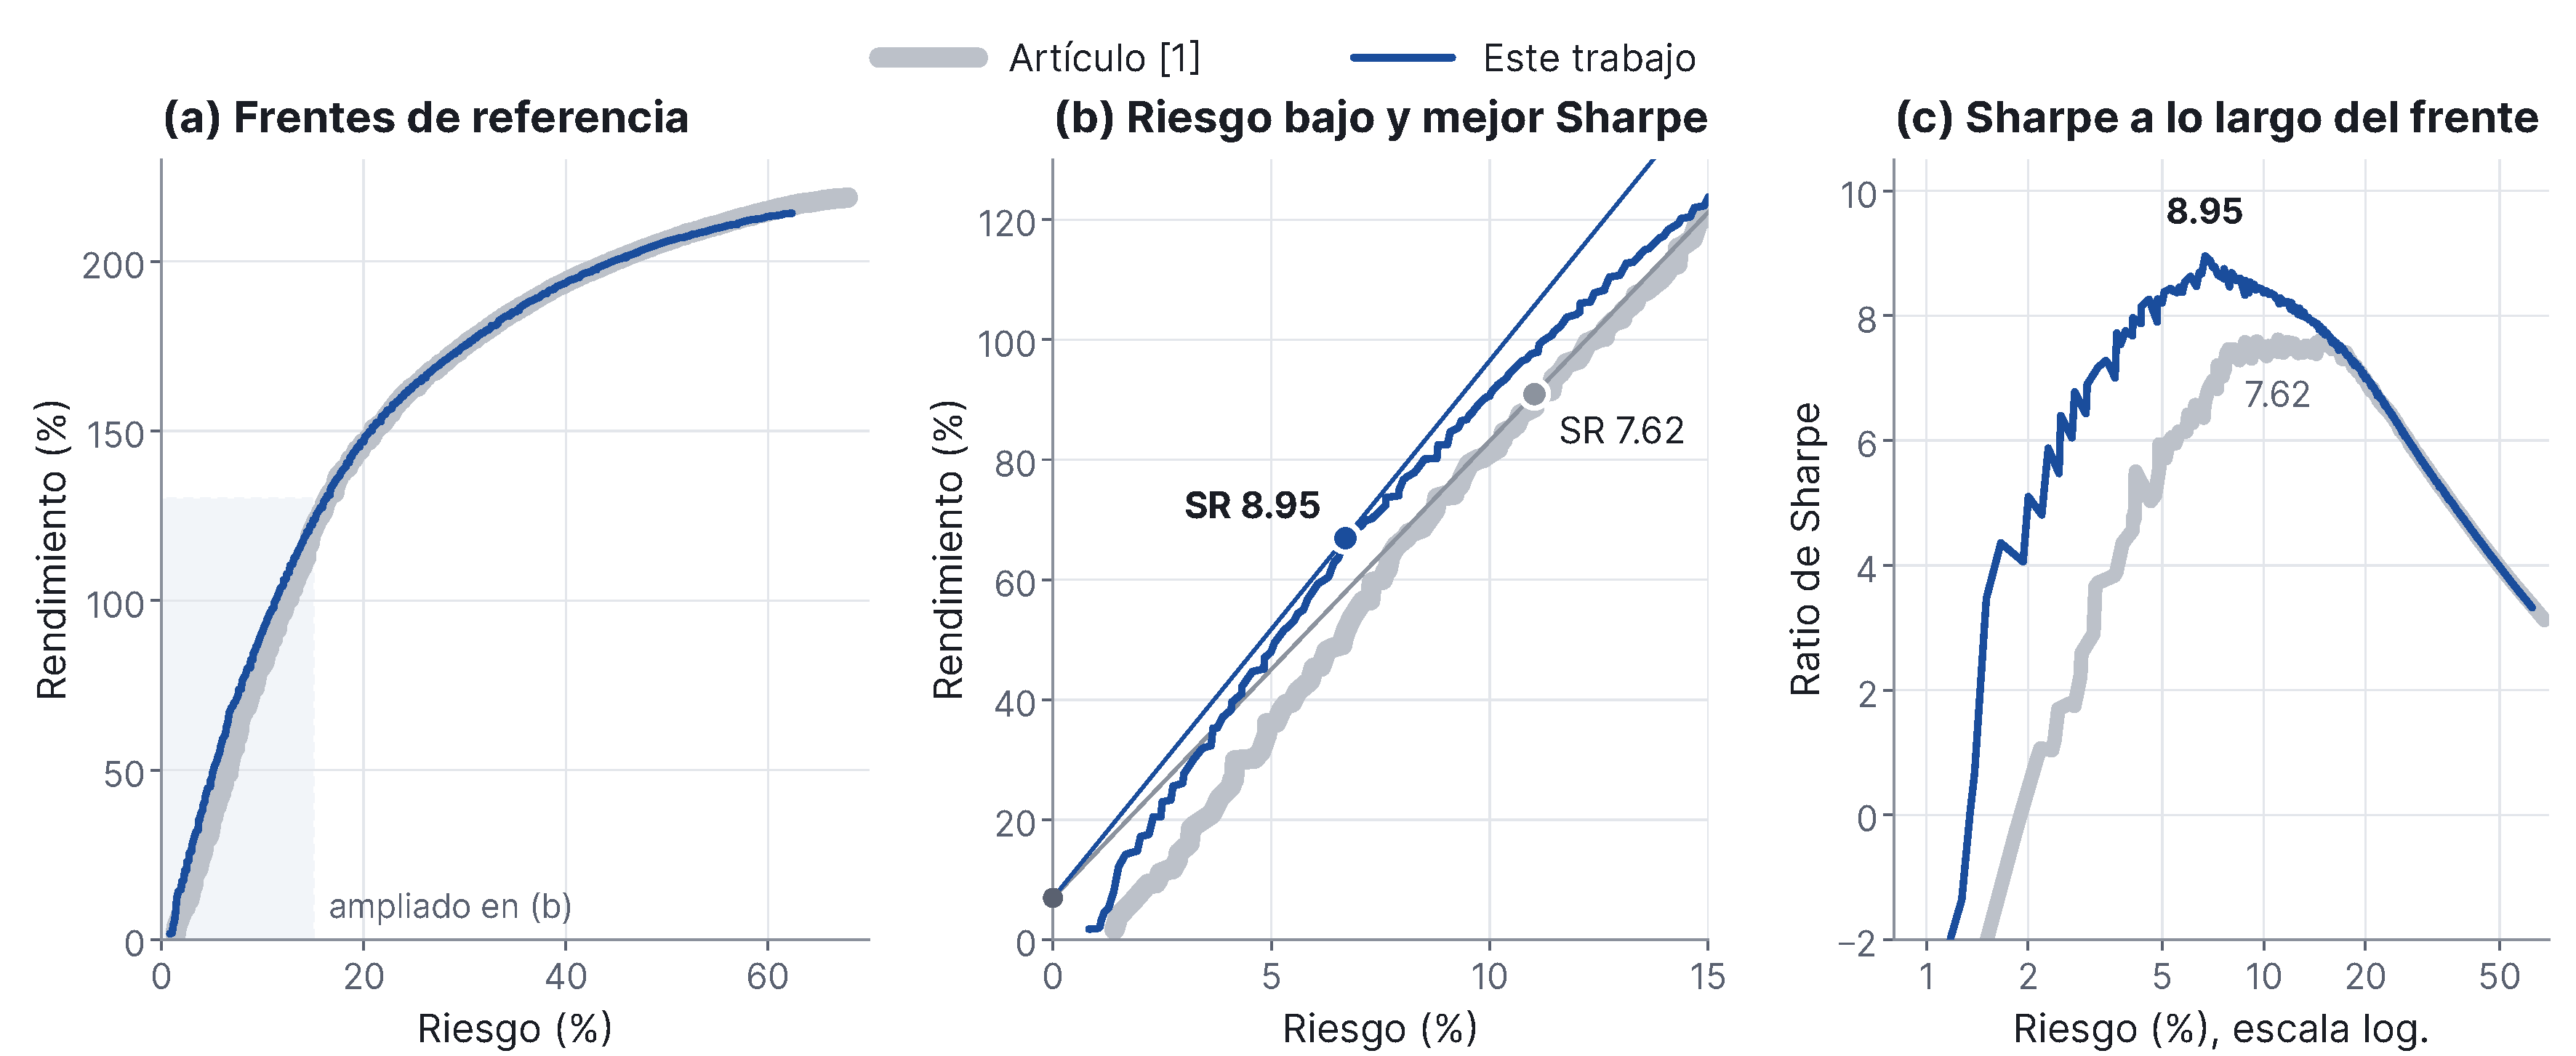
\includegraphics[width=600mm]{figures/fig_all20_6000_es.pdf}\par
    \vspace{2mm}
    {\smalltext\color{muted}(b) Las rectas desde la tasa libre de riesgo $R_f=6.97\,\%$ tocan cada frente en su
    mejor ratio de Sharpe $\mathrm{SR}=(R-R_f)/\sigma$, su pendiente. (c) Ratio de Sharpe de cada cartera del frente.\par}
  \end{minipage}%
  \hspace{20mm}%
  \begin{minipage}[t]{173mm}
    \vspace{0pt}
    \stat{8.95}{mejor ratio de Sharpe}{artículo 7.62 (+18\,\%)}\par\vspace{8mm}
    \stat{+12 p.\,p.}{rendimiento con 5\,\% de riesgo}{48\,\% vs 36\,\%}\par\vspace{8mm}
    \stat{0.82\,\%}{riesgo mínimo}{artículo 1.41\,\%}\par\vspace{8mm}
    \stat{0.951}{hipervolumen}{artículo 0.944}
  \end{minipage}

  \vspace{8mm}
  La mejora está bajo el 15\,\% de riesgo, donde 20 pesos son difíciles de evolucionar; por encima los frentes
  coinciden (extremo superior: 214\,\% frente a 219\,\%).
\end{minipage}

\vspace{\rowgap}
% ------------------------------------------------------------------------------------- fila 3
\hspace*{24mm}%
\begin{minipage}[t]{\colw}\body
  \sect{4}{La mejora crece con $N$}
  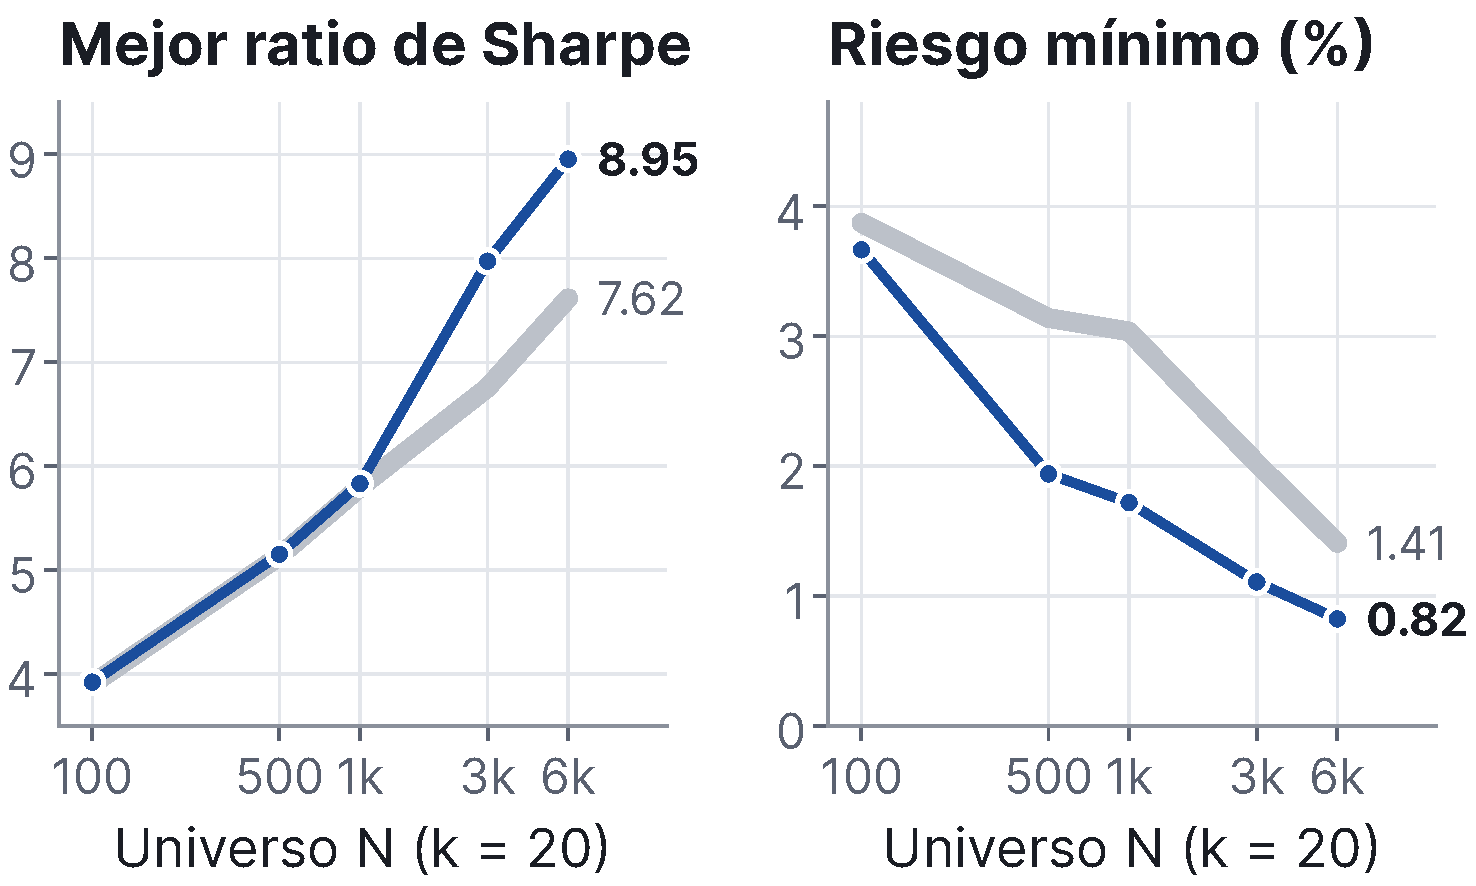
\includegraphics[width=\colw]{figures/fig_scaling_es.pdf}\par
  \vspace{4mm}
  Mejor hipervolumen e IGD+ en las cinco instancias de 20 activos; la mejora del Sharpe se dispara con
  $N\ge 3000$. En las instancias de 5 activos los frentes coinciden.
\end{minipage}%
\hspace{\gap}%
\begin{minipage}[t]{\colw}\body
  \sect{5}{Robustez y costo}
  \begin{itemize}
    \item \textbf{Por ejecución}, en las 12 instancias: hipervolumen significativamente mejor que el de la
    réplica en 33 de 36 pares algoritmo--instancia, nunca peor (Wilcoxon, 5\,\%). El artículo solo publica
    frentes combinados.
    \item \textbf{3 empates}, todos en los universos mayores (SMS-EMOA en ALL\_20\_3000 y ALL\_20\_6000,
    NSGA-II en ALL\_20\_6000). Ahí cada ejecución llega a menos riesgo, pero a un extremo de alto rendimiento
    más corto: la mutación elige al azar entre 6\,000 activos.
    \item \textbf{Costo}: mismo presupuesto de evaluaciones. Los QP subieron el tiempo de las 360 ejecuciones de
    63 a 67 min.
  \end{itemize}
\end{minipage}%
\hspace{\gap}%
\begin{minipage}[t]{\colw}\body
  \sect{6}{Fuera de muestra: 2024}
  Ambos frentes de ALL\_20\_6000 con precios de Yahoo Finance: carteras con el 80\,\% de su peso cotizado en
  2023--24, sin las de Sharpe negativo en ambos años.

  \vspace{3mm}
  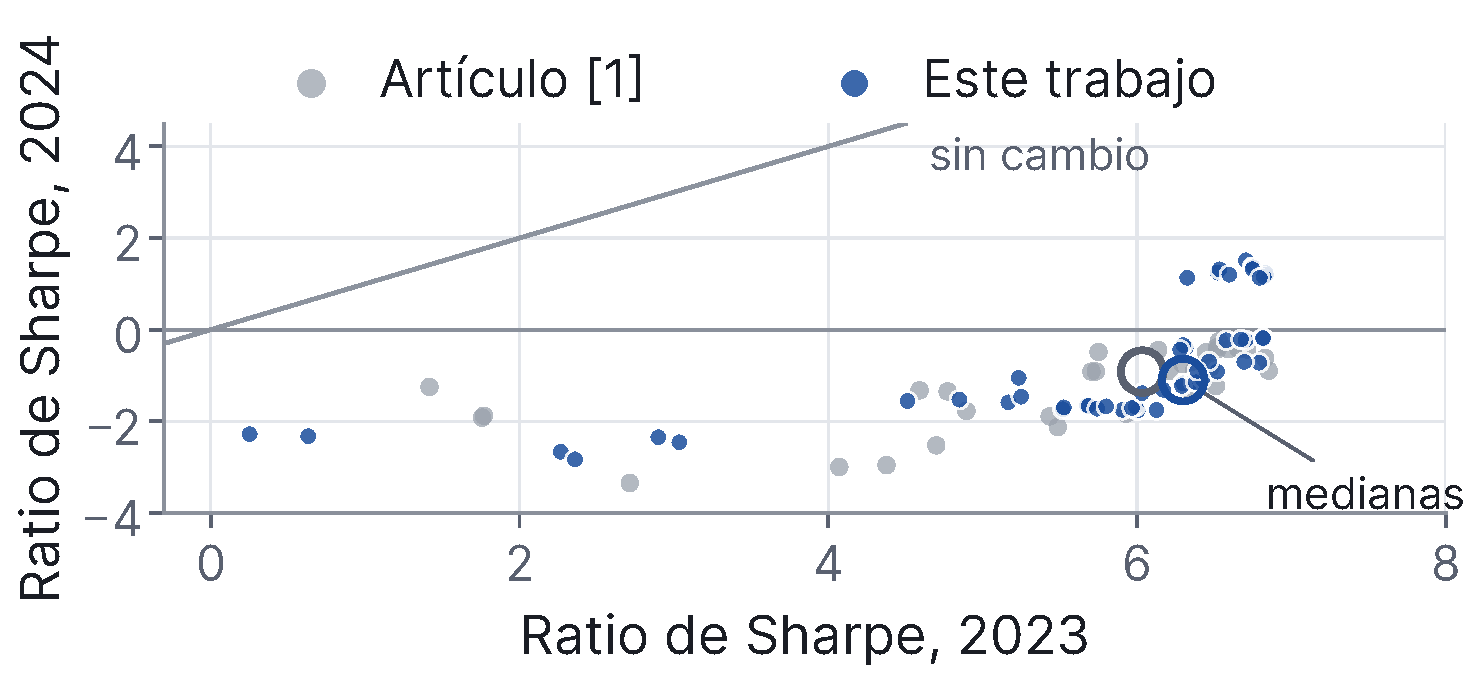
\includegraphics[width=\colw]{figures/fig_oos_es.pdf}\par
  \vspace{3mm}
  Mediana del Sharpe 2023 $\to$ 2024: 6.03 $\to$ $-0.91$ (artículo, 32 de 658 carteras) y 6.30 $\to$ $-1.10$
  (este trabajo, 54 de 369). Mejora de optimización, no de pronóstico.
\end{minipage}

\vspace{\rowgap}
% ------------------------------------------------------------------------------------- fila 4
\hspace*{24mm}%
\begin{minipage}[t]{\wide}\body
  \plainsect{Conclusiones}
  \begin{itemize}
    \item Una réplica en pymoo reproduce el orden de los algoritmos y los frentes de referencia del artículo.
    \item Evolucionar solo los activos (codificación por conjuntos, cruce por posiciones, mutación por
    intercambio, reparación HRP) y resolver los pesos con un QP da el mejor frente en todas las instancias de
    20 activos, y la mejora crece con $N$: en ALL\_20\_6000 el mejor ratio de Sharpe pasa de 7.62 a 8.95 con el
    mismo presupuesto.
    \item La mejora es dentro de muestra: en 2024 ambos enfoques pierden casi todo su ratio de Sharpe. El
    siguiente paso son mejores estimaciones de rendimiento y riesgo, más que un mejor optimizador.
  \end{itemize}
\end{minipage}%
\hspace{\gap}%
\begin{minipage}[t]{\colw}\fontsize{18pt}{23pt}\selectfont\raggedright
  \plainsect{Referencias}
  \vspace{-2mm}
  \begin{enumerate}[label={[\arabic*]}, leftmargin=1.8em, itemsep=2mm, topsep=0mm]
    \item A.\,J. Hidalgo-Marín, A.\,J. Nebro, J. García-Nieto. Efficient Selection of Investment Portfolios in
    Real-World Markets: A Multi-Objective Optimization Approach. \emph{Algorithms} 2026, 19(1), 20.
    doi:10.3390/a19010020
    \item M. López de Prado. Building Diversified Portfolios that Outperform Out of Sample. \emph{J. Portfolio
    Management} 2016, 42(4), 59--69.
    \item D. Goldfarb, A. Idnani. A numerically stable dual method for solving strictly convex quadratic
    programs. \emph{Math. Programming} 1983, 27, 1--33.
    \item J. Blank, K. Deb. pymoo: Multi-Objective Optimization in Python. \emph{IEEE Access} 2020, 8,
    89497--89509.
  \end{enumerate}
\end{minipage}

\end{document}
